\subsection*{Matriz DOFA}
\addcontentsline{toc}{subsection}{Matriz DOFA}

La matriz DOFA (también conocida como matriz FODA, o matriz DAFO) es una herramienta de análisis estratégico usada dentro del ámbito empresarial y para la toma de decisiones. La siglas D.O.F.A. proviene de las iniciales de los cuatro elementos clave que se analizan en esta matriz, las cuales son las \textit{Debilidades, Oportunidades, Fortalezas y Amenazas}. 

\begin{figure}[H]
	\centering
	\includegraphics[width=12cm]{Imagenes/MatrizDOFAEjemplo.png}
	\caption[{Ejemplo de matriz DOFA.}]{\centering Ejemplo de matriz DOFA. \textit{Fuente:} Sitio Web: (Pasos para implementar fácilmente la matriz DOFA de tu negocio, Actualícese, 2023)} 
	\label{fig:matrizdofaejemplo}
\end{figure}

Cada elemento dentro de la matriz DOFA tiene el siguiente significado:

\begin{itemize}
	\item \textbf{Debilidades (D):} Representan los factores críticos internos que generan una desventaja competitiva o limitan el rendimiento operativo. En el contexto del proyecto, incluyen restricciones en recursos técnicos, carencia de experiencia específica en ciertos nichos de mercado o procesos que aún requieren optimización para alcanzar la eficiencia deseada.
	
	\item \textbf{Oportunidades (O):} Constituyen factores externos favorables que la organización puede capitalizar para su crecimiento. Estas incluyen tendencias emergentes en el consumo digital, avances tecnológicos en inteligencia artificial, cambios regulatorios que fomentan la inclusión financiera y la creciente demanda de servicios EdTech en la región.
	
	\item \textbf{Fortalezas (F):} Son las capacidades internas distintivas y los activos estratégicos que proporcionan una ventaja sólida. Se consideran fortalezas el dominio de tecnologías específicas (como microservicios o arquitecturas en la nube), la propiedad intelectual del contenido educativo y el diseño de experiencias de usuario personalizadas.
	
	\item \textbf{Amenazas (A):} Comprenden las variables externas que podrían comprometer la estabilidad o el éxito del modelo de negocio. Entre estas se encuentran la saturación del mercado por competidores globales, la volatilidad macroeconómica, fluctuaciones en las tasas de interés y cambios abruptos en los hábitos de consumo de los usuarios.
\end{itemize}

Con esta definición, se inicia la construcción de los distintos aspectos de la empresa para lograr un análisis de aquella matriz en la figura \ref{fig:matrizdofaresultado}.

\begin{figure}[H]
	\centering
	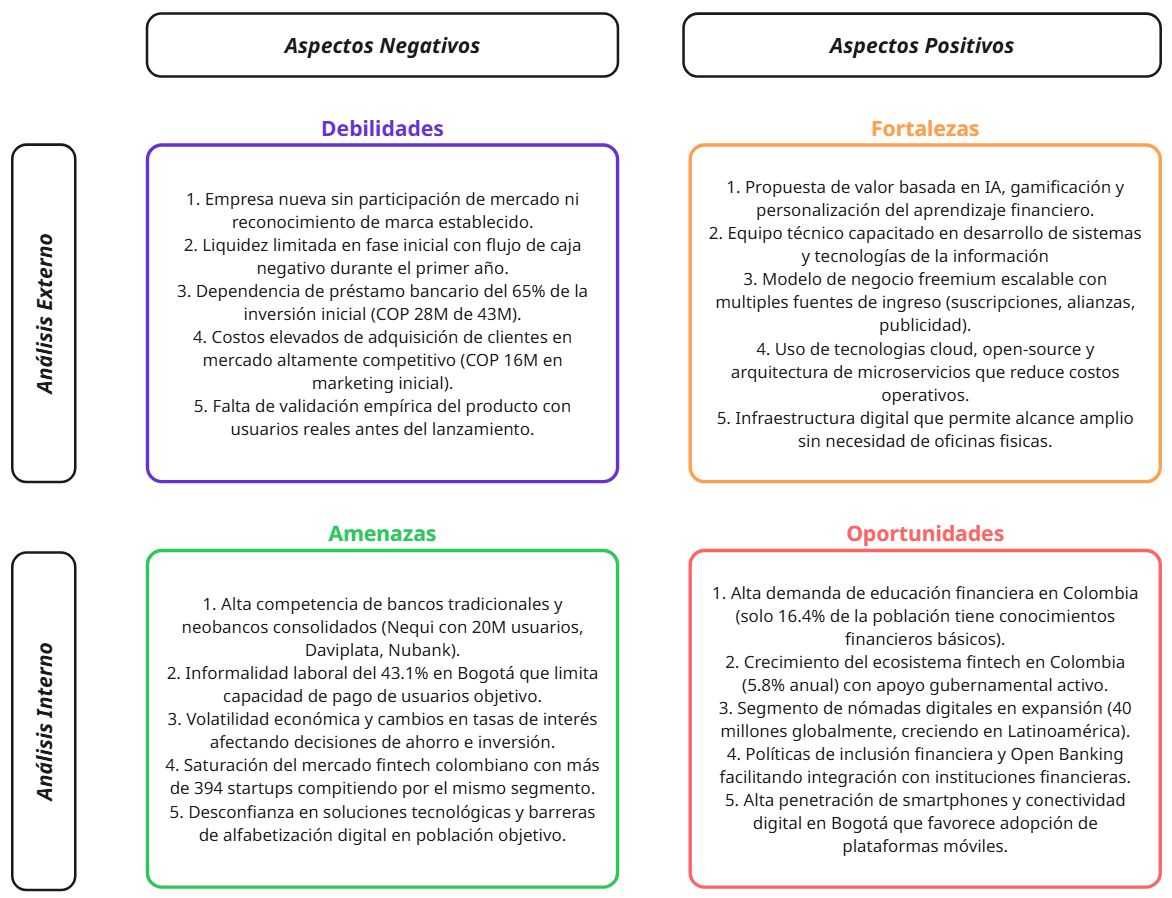
\includegraphics[width=15cm]{Imagenes/ResultadoMatrizDOFA.png}
	\caption[{Resultado de matriz DOFA.}]{\centering Resultado de matriz DOFA. \textit{Fuente:} Autores.} 
	\label{fig:matrizdofaresultado}
\end{figure}